% Typeset edition of prd.md
% Build: lualatex prd.tex
\documentclass[11pt]{article}

\usepackage{fontspec}
\usepackage{unicode-math}
\setmainfont{Libertinus Serif}
\setsansfont{Libertinus Sans}
\setmonofont{Libertinus Mono}[Scale=0.92]
\setmathfont{Libertinus Math}

\usepackage[a4paper, margin=2.35cm]{geometry}
\usepackage{microtype}
\usepackage{amsmath}
\usepackage{booktabs}
\usepackage{array}
\usepackage{enumitem}
\usepackage{graphicx}
\usepackage{xcolor}
\usepackage[most]{tcolorbox}
\usepackage{tikz}
\usetikzlibrary{arrows.meta, positioning, fit, backgrounds}

\usepackage[
  colorlinks=true,
  linkcolor=cyanlayer,
  urlcolor=cyanlayer,
  citecolor=cyanlayer,
  pdftitle={PRD: A two-layer MNIST network},
  pdfauthor={Vincent}
]{hyperref}

\definecolor{ink}{HTML}{1C2430}
\definecolor{muted}{HTML}{5C6778}
\definecolor{cyanlayer}{HTML}{0E7490}
\definecolor{violetlayer}{HTML}{6D28D9}
\definecolor{sand}{HTML}{F6F1E8}
\definecolor{coral}{HTML}{C2410C}
\definecolor{line}{HTML}{E6DFD4}

\pagecolor{white}
\color{ink}
\setlist[itemize]{leftmargin=1.25em, itemsep=0.28em, topsep=0.35em}
\setlist[enumerate]{leftmargin=1.35em, itemsep=0.32em, topsep=0.4em}
\renewcommand{\arraystretch}{1.18}

\tcbset{
  prd/.style={
    colback=sand,
    colframe=line,
    coltitle=ink,
    boxrule=0.6pt,
    arc=1.5pt,
    left=9pt, right=9pt, top=7pt, bottom=7pt,
    fonttitle=\sffamily\bfseries\small,
  }
}

\newcommand{\pill}[2]{%
  \tcbox[on line, colback=#1!12, colframe=#1!45, boxrule=0.4pt,
         arc=2pt, left=4pt, right=4pt, top=1.5pt, bottom=1.5pt,
         fontupper=\sffamily\bfseries\scriptsize\color{#1!80!black}]{#2}%
}

% ---------------------------------------------------------------------------
% Structure figure: 28×28 image → 784 → 32 ReLU → 10 sigmoid
% Drawn nodes are a readable sample. The nets are fully connected.
% ---------------------------------------------------------------------------
\newcommand{\NetworkDiagram}{%
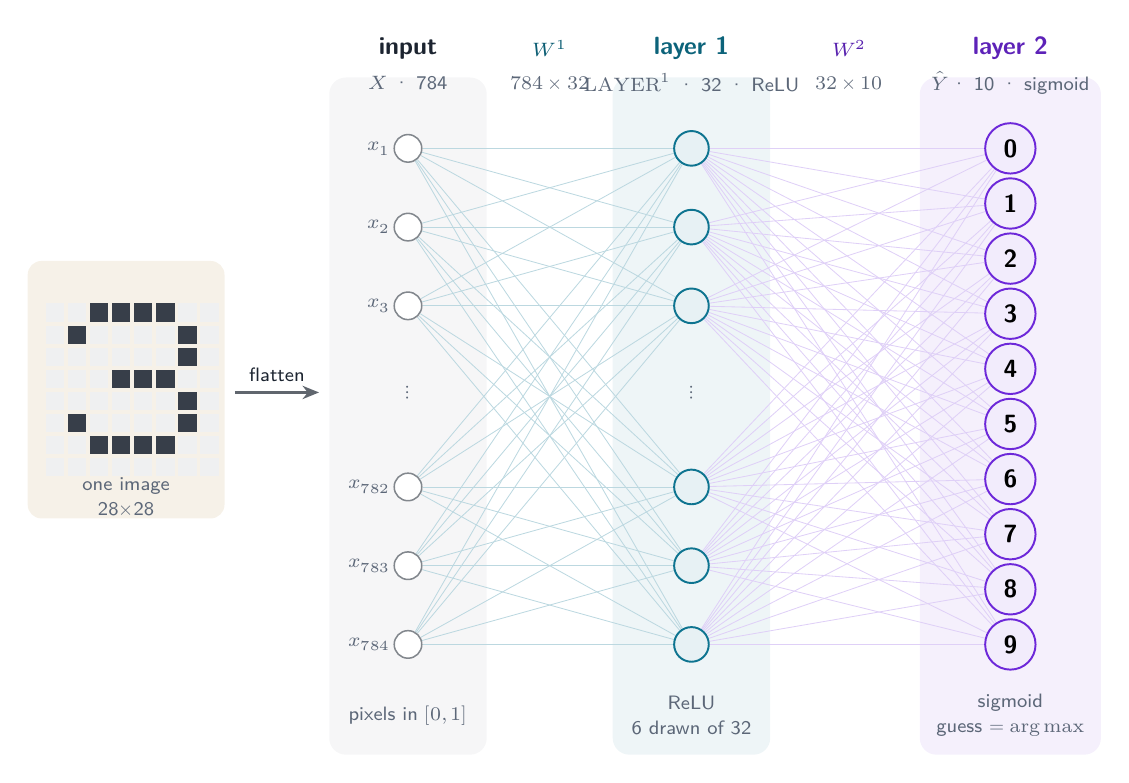
\begin{tikzpicture}[
  x=1cm, y=1cm,
  >={Stealth[length=2.1mm, width=1.7mm]},
  innode/.style={
    circle, draw=ink!55, fill=white, line width=0.55pt,
    minimum size=3.5mm, inner sep=0pt
  },
  hnode/.style={
    circle, draw=cyanlayer, fill=cyanlayer!10, line width=0.7pt,
    minimum size=4.4mm, inner sep=0pt
  },
  onode/.style={
    circle, draw=violetlayer, fill=violetlayer!9, line width=0.7pt,
    minimum size=6.4mm, inner sep=0pt,
    font=\sffamily\bfseries\small
  },
  lbl/.style={font=\scriptsize\color{muted}, inner sep=1pt},
  head/.style={font=\sffamily\bfseries\small, text=ink},
  sub/.style={font=\sffamily\scriptsize, text=muted},
]

% --- plates behind each column ---
\begin{scope}[on background layer]
  \fill[sand, rounded corners=5pt] (-1.28,-1.55) rectangle (1.22,1.72);
  \fill[ink!4, rounded corners=6pt] (2.55,-4.55) rectangle (4.55,4.05);
  \fill[cyanlayer!7, rounded corners=6pt] (6.15,-4.55) rectangle (8.15,4.05);
  \fill[violetlayer!7, rounded corners=6pt] (10.05,-4.55) rectangle (12.35,4.05);
\end{scope}

% --- 8×8 stand-in for the 28×28 digit (a handwritten 3) ---
\begin{scope}[shift={(-1.05,1.18)}]
  \pgfmathsetmacro{\cs}{0.28}
  \pgfmathsetmacro{\side}{0.235}
  \foreach \r in {0,...,7} {
    \foreach \c in {0,...,7} {
      \fill[ink!7] (\c*\cs, -\r*\cs) rectangle ++(\side, -\side);
    }
  }
  \foreach \c/\r in {2/0, 3/0, 4/0, 5/0, 1/1, 6/1, 6/2, 3/3, 4/3, 5/3, 6/4, 1/5, 6/5, 2/6, 3/6, 4/6, 5/6} {
    \fill[ink!88] (\c*\cs, -\r*\cs) rectangle ++(\side, -\side);
  }
\end{scope}
\node[sub, align=center] at (-0.03,-1.28) {one image\\[1pt]28$\times$28};

% --- input sample ---
\node[head] at (3.55, 4.42) {input};
\node[sub] at (3.55, 3.98) {$X$ \textperiodcentered\ 784};
\node[innode, label={[lbl]left:$x_{1}$}] (x1) at (3.55, 3.15) {};
\node[innode, label={[lbl]left:$x_{2}$}] (x2) at (3.55, 2.15) {};
\node[innode, label={[lbl]left:$x_{3}$}] (x3) at (3.55, 1.15) {};
\node[lbl] (xv) at (3.55, 0.05) {$\vdots$};
\node[innode, label={[lbl]left:$x_{782}$}] (x5) at (3.55,-1.15) {};
\node[innode, label={[lbl]left:$x_{783}$}] (x6) at (3.55,-2.15) {};
\node[innode, label={[lbl]left:$x_{784}$}] (x7) at (3.55,-3.15) {};
\node[sub] at (3.55,-4.05) {pixels in $[0,1]$};

\draw[->, line width=0.8pt, draw=ink!70]
  (1.35, 0.05) -- node[above, font=\sffamily\scriptsize, text=ink] {flatten}
  (2.42, 0.05);

% --- hidden sample (8 of 32) ---
\node[head, text=cyanlayer!85!black] at (7.15, 4.42) {layer 1};
\node[sub] at (7.15, 3.98) {$\mathrm{LAYER}^{1}$ \textperiodcentered\ 32 \textperiodcentered\ ReLU};
\node[hnode] (h1) at (7.15, 3.15) {};
\node[hnode] (h2) at (7.15, 2.15) {};
\node[hnode] (h3) at (7.15, 1.15) {};
\node[lbl] at (7.15, 0.05) {$\vdots$};
\node[hnode] (h4) at (7.15,-1.15) {};
\node[hnode] (h5) at (7.15,-2.15) {};
\node[hnode] (h6) at (7.15,-3.15) {};
\node[sub, align=center] at (7.15,-4.05) {ReLU\\[1pt]6 drawn of 32};

% --- output: all 10 digits ---
\node[head, text=violetlayer!85!black] at (11.2, 4.42) {layer 2};
\node[sub] at (11.2, 3.98) {$\hat{Y}$ \textperiodcentered\ 10 \textperiodcentered\ sigmoid};
\foreach \d in {0,...,9} {
  \pgfmathsetmacro{\yy}{3.15 - \d*0.70}
  \node[onode] (o\d) at (11.2, \yy) {\d};
}
\node[sub, align=center] at (11.2,-4.05) {sigmoid\\[1pt]guess $=\arg\max$};

% --- bundles: fully connected between the nodes we drew ---
\begin{scope}[on background layer]
  \foreach \a in {1,2,3,5,6,7} {
    \foreach \b in {1,...,6} {
      \draw[cyanlayer!28, line width=0.3pt] (x\a) -- (h\b);
    }
  }
  \foreach \b in {1,...,6} {
    \foreach \d in {0,...,9} {
      \draw[violetlayer!22, line width=0.3pt] (h\b) -- (o\d);
    }
  }
\end{scope}

% Weight names sit in the gaps, on the same row as the column titles.
\node[font=\sffamily\bfseries\scriptsize, text=cyanlayer!80!black] at (5.35, 4.42) {$W^{1}$};
\node[sub] at (5.35, 3.98) {$784\times 32$};
\node[font=\sffamily\bfseries\scriptsize, text=violetlayer!80!black] at (9.15, 4.42) {$W^{2}$};
\node[sub] at (9.15, 3.98) {$32\times 10$};

\end{tikzpicture}%
}

\newcommand{\NeuronDiagram}{%
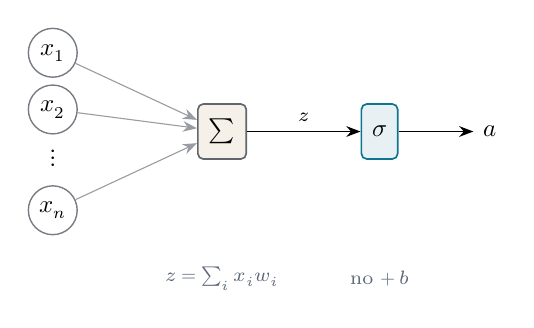
\begin{tikzpicture}[
  x=1cm, y=1cm,
  >={Stealth[length=1.8mm]},
  font=\small,
  pin/.style={circle, draw=ink!60, fill=white, minimum size=6.2mm, inner sep=0pt, line width=0.5pt},
  box/.style={rounded corners=2pt, draw=ink!70, fill=sand, line width=0.6pt,
              minimum height=7mm, inner sep=4pt, font=\small},
]
  \node[pin] (x1) at (0, 0.72) {$x_{1}$};
  \node[pin] (x2) at (0, 0) {$x_{2}$};
  \node at (0,-0.62) {$\vdots$};
  \node[pin] (xn) at (0,-1.28) {$x_{n}$};
  \node[box] (sum) at (2.15,-0.28) {$\sum$};
  \node[box, fill=cyanlayer!10, draw=cyanlayer] (act) at (4.15,-0.28) {$\sigma$};
  \node[font=\small] (a) at (5.55,-0.28) {$a$};
  \draw[->, ink!45] (x1) -- (sum);
  \draw[->, ink!45] (x2) -- (sum);
  \draw[->, ink!45] (xn) -- (sum);
  \draw[->, line width=0.7pt] (sum) -- node[above, font=\scriptsize] {$z$} (act);
  \draw[->, line width=0.7pt] (act) -- (a);
  \node[font=\scriptsize, text=muted] at (2.15,-2.15) {$z=\sum_{i} x_{i} w_{i}$};
  \node[font=\scriptsize, text=muted] at (4.15,-2.15) {no $+\,b$};
\end{tikzpicture}%
}

\begin{document}

% ----- title -----
\noindent
{\sffamily\color{cyanlayer}\bfseries\small PRODUCT REQUIREMENTS}
\hfill
\pill{cyanlayer}{implemented}\quad
\pill{muted}{pure Python}

\vspace{0.55em}
{\sffamily\bfseries\fontsize{26}{30}\selectfont A two-layer MNIST network\par}
\vspace{0.35em}
{\large\color{muted} How a small net turns 784 pixels into a digit, written so the code can follow the math.\par}

\vspace{0.7em}
{\color{line}\hrule height 0.8pt}
\vspace{0.9em}

\noindent
\begin{tabular}{@{}l l@{}}
\sffamily\small\color{muted} Source & \texttt{prd.md}, typeset here as \texttt{prd.tex} \\[2pt]
\sffamily\small\color{muted} Code & \texttt{two\_layer\_mnist.py} \\[2pt]
\sffamily\small\color{muted} Stories & \texttt{user-stories.md} \\[2pt]
\sffamily\small\color{muted} Reader & Vincent, learning the mechanism by building it \\
\end{tabular}

\vspace{1.15em}

\section*{Problem}

Vincent wants a very simple neural network in Python so he can learn how it works: a from-scratch two-layer MNIST network. In run mode he wants a clear view of both layers --- the 32 hidden neurons and the 10 output scores --- without the training-loss log.

The priority is that the loop is obvious. Accuracy is not a goal.

\section*{Goals}

\begin{itemize}
  \item A small, self-explanatory network in Python that makes the mechanics visible.
  \item The definition from Vincent's notes: 784 inputs, 32 hidden neurons, 10 outputs.
  \item Train on a small MNIST subset and print a few digit guesses.
  \item Run mode: once weights exist, show each test digit with \textsc{layer}\textsuperscript{1} and \textsc{layer}\textsuperscript{2}.
  \item Spec-driven: this document is the source of truth. It runs on Vincent's machine.
\end{itemize}

\section*{Non-goals}

\begin{itemize}
  \item Any language other than Python.
  \item Any ML library (PyTorch, TensorFlow, Keras, scikit-learn, JAX, and similar).
  \item NumPy or other numeric libraries. Pure Python only.
  \item The full 60{,}000\,/\,10{,}000 MNIST training set.
  \item Production OCR, GPUs, or a deep-learning framework.
  \item An accuracy target, a hyperparameter search, or tuning for a score.
\end{itemize}

\section*{Theory}

This is the teaching core. \texttt{two\_layer\_mnist.py} should read as a walk through of what follows.

\subsection*{What the network is}

A neural network here is not a black box. It is two tables of numbers (the weights) plus two small functions (the activations).

We show it a picture of a handwritten digit. It answers with 10 scores, one per digit $0,\ldots,9$. The largest score is its guess.

It does not see a picture the way we do. The picture becomes 784 numbers: each pixel of the $28\times 28$ grid is one number between 0 (white) and 1 (black), laid out in a single row. One image is a row of length 784. A training batch of 150 images is the matrix $X$ of shape $150\times 784$.

\subsection*{What we want to recognize}

The goal is not a full page and not a printed font. Given one small handwritten numeral, name the digit.

\begin{figure}[ht]
  \centering
  \setlength{\tabcolsep}{8pt}
  \begin{tabular}{cccccc}
    
\includegraphics[width=1.85cm]{mnist-examples/digit-0.png} &
    
\includegraphics[width=1.85cm]{mnist-examples/digit-1.png} &
    
\includegraphics[width=1.85cm]{mnist-examples/digit-2.png} &
    
\includegraphics[width=1.85cm]{mnist-examples/digit-3.png} &
    
\includegraphics[width=1.85cm]{mnist-examples/digit-7.png} &
    
\includegraphics[width=1.85cm]{mnist-examples/digit-8.png} \\[4pt]
    \sffamily\small 0 &
    \sffamily\small 1 &
    \sffamily\small 2 &
    \sffamily\small 3 &
    \sffamily\small 7 &
    \sffamily\small 8 \\
  \end{tabular}
  \caption{Real MNIST digits from this project. The caption is the true label: what the network should guess after it looks at the picture.}
\end{figure}

Handwriting varies --- a sloppy 7 against a crossed 7, an 8 that looks like a 0. That is why training uses many examples. After training we print a few guesses next to labels like these. We do not require a score. We want the loop to be obvious.

\subsection*{A neuron}

One neuron does two things.

\begin{enumerate}
  \item \textbf{Weighted sum.} Multiply each incoming number by a weight and add the products. That sum is $z$.
  \item \textbf{Activation.} Pass $z$ through a small function $\sigma(z)$ so the output stays in a useful range.
\end{enumerate}

The weights are the knobs we learn. They start random. After training they should push the digit scores toward the labels.

This project has no bias terms. There is no extra $+\,b$ on a neuron, so the theory stays aligned with the two weight matrices only.

\begin{figure}[ht]
  \centering
  \NeuronDiagram
  \caption{One neuron. The weighted sum $z$ is sent through $\sigma$. Hidden neurons use ReLU; output neurons use the sigmoid. Nothing is added after the sum.}
\end{figure}

\subsection*{Two layers}

\begin{itemize}
  \item \textbf{Layer 1, hidden.} 32 neurons. Each one looks at all 784 pixels. Together they are a 32-number internal sketch of the image: not a digit yet, just features the second layer can use.
  \item \textbf{Layer 2, output.} 10 neurons. Each one looks at those 32 numbers and votes for one digit.
\end{itemize}

There is one hidden layer and one output layer --- two layers in total. ``Both layers'' in run mode means \textsc{layer}\textsuperscript{1} and \textsc{layer}\textsuperscript{2}, not two hidden layers.

\begin{figure}[ht]
  \centering
  \NetworkDiagram
  \caption{Structure of the network. The grid stands for one $28\times 28$ digit, flattened into the 784-vector $X$. Six input circles and six hidden circles are drawn so the picture stays readable; the real hidden layer has 32 neurons, and every input connects to every one of them. All ten output scores are drawn. $W^{1}$ and $W^{2}$ are the only learned tables. There is no bias.}
\end{figure}

The pale lines are the idea of a full connection, not a plot of individual weights. Shapes that actually multiply:

\begin{center}
\small
\begin{tabular}{@{}l l l@{}}
\toprule
\sffamily\bfseries object & \sffamily\bfseries meaning & \sffamily\bfseries shape \\
\midrule
$X$ & 150 images, 784 pixels each & $150\times 784$ \\
$W^{1}$ & weights of every hidden neuron & $784\times 32$ \\
$Z^{1}$ & hidden weighted sums & $150\times 32$ \\
$\mathrm{LAYER}^{1}$ & hidden activations & $150\times 32$ \\
$W^{2}$ & weights of every output neuron & $32\times 10$ \\
$Z^{2}$ & output weighted sums & $150\times 10$ \\
$\hat{Y}$ & 10 scores per image & $150\times 10$ \\
$Y$ & true labels, one-hot & $150\times 10$ \\
\bottomrule
\end{tabular}
\end{center}

The notes label $W^{1}$ as $32\times 150$ and $W^{2}$ as $10\times 150$. Those sizes do not multiply with $X$ ($150\times 784$). We keep the 32 and the 10 neurons, and we use $784\times 32$ and $32\times 10$ so the products are valid.

\subsection*{Forward pass}

The schema, with $\sigma$ meaning ``an activation'' in general:

\begin{tcolorbox}[prd, title=Forward schema]
\[
X \rightarrow \otimes W^{1} \rightarrow Z^{1} \rightarrow \sigma \rightarrow \mathrm{LAYER}^{1}
\rightarrow \otimes W^{2} \rightarrow Z^{2} \rightarrow \sigma \rightarrow \hat{Y}
\;\gg\; \mathrm{LOSS}(\hat{Y}, Y)
\]
\end{tcolorbox}

In this project the two activations are different functions.
\begin{align*}
Z^{1} &= X W^{1} \\
\mathrm{LAYER}^{1} &= \mathrm{ReLU}(Z^{1}) \\
Z^{2} &= \mathrm{LAYER}^{1}\, W^{2} \\
\hat{Y} &= \mathrm{sigmoid}(Z^{2})
\end{align*}

\textbf{ReLU}, on the hidden layer. $\mathrm{ReLU}(z)=\max(0,z)$. Negative sums become 0; positive sums pass through. The slope is 1 when $z>0$, and 0 otherwise.

\textbf{Sigmoid}, on the output layer.
\[
\mathrm{sigmoid}(z)=\frac{1}{1+e^{-z}}.
\]
Each of the 10 numbers is squashed into $(0,1)$ and treated as a soft score for that digit. They are not forced to sum to 1 (that would be softmax, which is out of scope). The guess is $\arg\max$: the column with the largest score.

\subsection*{Loss}

The true label is a one-hot row. Digit 3 is $(0,0,0,1,0,0,0,0,0,0)$.

Mean squared error compares every score with every one-hot entry:
\[
\mathrm{LOSS}=(\hat{Y}-Y)^{2},
\]
summed over the batch in the code. If the network is sure about the right digit, $\hat{Y}$ is close to $Y$ and the loss is small. If it is sure about the wrong digit, the loss is large.

We do not chase an accuracy percentage. The loss exists so the backward pass has a number to reduce.

\subsection*{Backward pass}

Learning is backpropagation plus SGD. Measure the error at the output, send it backward through each layer, and nudge every weight a little so the next forward pass is less wrong.

The derivatives we need:
\begin{align*}
\mathrm{sigmoid}'(z) &= \sigma(z)\,(1-\sigma(z)), \\
\mathrm{ReLU}'(z) &=
  \begin{cases}
    1 & \text{if } z>0,\\
    0 & \text{otherwise.}
  \end{cases}
\end{align*}
$\odot$ is element-wise multiply. The dot is matrix multiply. $(\,\cdot\,)^{\!\top}$ is transpose.

For one batch:
\begin{enumerate}
  \item Error at the output (MSE composed with the sigmoid):
  \[
    E = 2(\hat{Y}-Y)\odot \mathrm{sigmoid}'(Z^{2}).
  \]
  \item How the second-layer weights should change:
  \[
    \frac{\partial \mathrm{LOSS}}{\partial W^{2}} = (\mathrm{LAYER}^{1})^{\!\top} E.
  \]
  For each of the 32 hidden values: how much did it push each of the 10 output errors?
  \item Send that error back through $W^{2}$ and through ReLU:
  \[
    \frac{\partial \mathrm{LOSS}}{\partial W^{1}}
      = X^{\!\top}\!\left(\bigl(E\,(W^{2})^{\!\top}\bigr)\odot \mathrm{ReLU}'(Z^{1})\right).
  \]
  For each of the 784 pixels: how much did it push each of the 32 hidden neurons, given the error that arrived from the output?
  \item SGD step, with learning rate $\eta=1$:
  \[
    W^{1} \leftarrow W^{1}-\eta\,\frac{\partial \mathrm{LOSS}}{\partial W^{1}},
    \qquad
    W^{2} \leftarrow W^{2}-\eta\,\frac{\partial \mathrm{LOSS}}{\partial W^{2}}.
  \]
\end{enumerate}

No momentum, no Adam, no regularization. A \textbf{batch} is 150 images. An \textbf{epoch} is one walk through the about 1{,}000 training images (about seven batches). Training runs for 50 epochs.

One practical note lives next to the update in the code. The formulas above differentiate a \emph{summed} MSE. That sum, over a $150\times 10$ batch, is far too large for $\eta=1$ (the sigmoid saturates in a single step). The code divides the gradients by $\text{batch}\times 10$, so the step is mean MSE while the printed loss stays the summed number.

\section*{Model definition}

150 observations in a matrix $X$ of shape $150\times 784$: 150 rows, 784 columns.

Two weight matrices. The notes write $W^{1}$ as $32\times 150$ and $W^{2}$ as $10\times 150$. The locked shapes are $W^{1}\in\mathbb{R}^{784\times 32}$ and $W^{2}\in\mathbb{R}^{32\times 10}$.

Layers: a first layer of 32 neurons, a second layer of 10 neurons. The output has shape $150\times 10$, one column per digit class.

Hidden activation: ReLU. Output activation: sigmoid.

\section*{Decisions}

\begin{center}
\small
\begin{tabular}{@{}>{\sffamily\bfseries}l p{11.4cm}@{}}
\toprule
Language & Python, standard library only. \\
Purpose & Learn how a neural network works. \\
Stack & Pure Python, from scratch. No ML library and no NumPy. \\
Task & Handwritten digits on a MNIST subset. \\
Architecture & $784 \rightarrow 32 \rightarrow 10$. \\
Weights & $W^{1}$ is $784\times 32$. $W^{2}$ is $32\times 10$. No biases. \\
Predict & $\arg\max$ of the 10 sigmoid scores, a digit $0$--$9$. \\
Data & About 1{,}000 train images and 200 test images, in \texttt{mnist\_subset.json.gz}. \\
Batch & 150 images per step. \\
Epochs & 50. Print the loss after each epoch, in training mode only. \\
Step size & $\eta = 1$, on mean MSE (see the note in the backward pass). \\
Weights file & \texttt{mnist\_weights.json.gz}, so run mode can skip training. \\
Deliverable & One well-commented Python file: the theory, in code. \\
\bottomrule
\end{tabular}
\end{center}

\subsection*{Run mode}

Training mode is for watching the loss. Run mode is for seeing the network think.

\begin{itemize}
  \item \texttt{python3 two\_layer\_mnist.py --train} trains and saves the weights.
  \item \texttt{python3 two\_layer\_mnist.py --run} loads the weights and draws. No epoch log.
  \item With no flag, the file trains, saves, then runs.
\end{itemize}

For one test image of each digit $0,\ldots,9$, run mode:

\begin{enumerate}
  \item Draws the $28\times 28$ digit (sixel in Foot, text otherwise).
  \item Draws \textsc{layer}\textsuperscript{1}: the 32 ReLU values as a $4\times 8$ heat grid of fixed-width cells, plus a one-line sparkline. Cells are scaled to that image's peak ReLU.
  \item Draws \textsc{layer}\textsuperscript{2}: ten sigmoid bars, labeled $0$ through $9$. A star marks the guess. The true label and the guess use distinct highlights.
  \item Prints one line: guess against truth.
\end{enumerate}

Color is soft ANSI when stdout is a terminal. \texttt{NO\_COLOR} switches it off. No GUI toolkit.

\section*{Requirements}

\begin{itemize}
  \item From scratch, in pure Python: an explicit forward pass, loss, and backprop.
  \item Comments retell this theory next to the matching lines.
  \item No ML library, no NumPy, no other language.
  \item A MNIST subset file for training and for the guesses.
  \item Two layers, 32 then 10.
  \item One \texttt{.py} file, plus the modes above.
\end{itemize}

\section*{Success}

\begin{itemize}
  \item The Python file is simple enough to read as the forward, loss, backward, and update story.
  \item Training prints the loss each epoch and saves the weights.
  \item Run mode loads those weights and shows each sample digit with both layers.
  \item No accuracy number is required, and we do not tune toward one.
\end{itemize}

\section*{Constraints}

Python, standard library only, on Vincent's machine. The path is this PRD, then the user stories, then \texttt{two\_layer\_mnist.py}.

\section*{Open questions}

None.

\vspace{1.4em}
{\color{line}\hrule height 0.6pt}
\vspace{0.55em}
{\sffamily\scriptsize\color{muted} Typeset from \texttt{docs/prd.md}. The network figure shows a sample of the connections; the implemented net is fully connected, $784\rightarrow 32\rightarrow 10$, with ReLU then sigmoid and no biases.}

\end{document}
